\section{Continuous Query-Based Syndication}

Continuous Query-Based Syndication (CQBS) is a hybrid publish-subscribe pattern that provides the expressiveness of content-based systems while retaining the simplicity of topic-based systems.
The goal of CQBS is to provide a messaging system that can account for and adapt to the heterogeneity of data sources in the IoT.
CQBS endows embedded publishers to describe themselves using rich metadata, and provides subscribers to discover and subscribe to relevant data sources and maintain a consistent view of the context of those sources.

Here, we first establish the CQBS primitives --- streams and metadata --- before delving into how CQBS operates and what roles publishers and subscribers play.
We then describe the design and implementation of an individual broker (we defer the discussion of the full distributed system to Section~\ref{section:coordinator}.

\begin{figure}
\centering
\begin{lstlisting}[language=pseudocode,basicstyle=\small]
UUID = "dd9ef92e-140a-11e6-b352-1002b58053c7"
# register client
metadata = {
  UUID = UUID,
  Location/Room = "410",
  Location/Building = "Soda",
  Location/City = "Berkeley",
  Point/Type = "Sensor",
  Point/Measure = "Temperature"
  UnitofMeasure = "Fahrenheit",
  UnitofTime = "ms",
  Timezone = "America/Los_Angeles"
}
register_msg := msgpack.encode(metadata)
send_to_broker(register_msg)
while True:
    temp_val := read_sensor()
    msg := msgpack.encode({
            UUID = UUID,
            Value = temp_val
           })
    send_to_broker(msg)
    sleep(10)
\end{lstlisting}
\caption{Client registration and publishing pseudocode}
\label{fig:pseudoclient}
\end{figure}

\subsection{Streams and Metadata}

A stream is a virtual representation of a specific sensor or actuator channel (a ``capability'') that is indexed by a 16-byte universally unique identifier (UUID).
Each stream is described by \emph{metadata}, which is a bag of key-value pairs: keys are required to be string, but values may be any one-dimensional data type\footnote{In our implementation, values are restricted to strings: see Section~\ref{section:evaluation}.}.
Key-value pairs are most effective when drawn from some well-known ontology (such as Semantic Sensor Web~\cite{sheth2008semantic}), but our system places no restrictions on their content.
The association of metadata to a stream is done by the UUID; when a publisher creates a new stream, it registers that stream with the broker by sending a message containing the UUID and all of the metadata.
The broker (or the coordinator, in the distributed case) stores the mapping from stream UUID to metadata.
A publisher changes metadata by sending the ``diff'' of which keys and values have changed.
A given producer (data provider) can have as many streams as it wishes.
Each message contains at least the UUID of the originating stream, and can also contain any metadata changes, and of couse the published value itself, which can be any serializable object.

An example of metadata for a temperature sensor, and the basic client logic, can be found in Figure~\ref{fig:pseudoclient}.
In the initial registration message, along with the other metadata, the reporting process describes the thermostat as being in room 410 Soda.
If this changes, such as if the sensor were on a piece of smart clothing or furniture, the sensor attaches the metadata update \lstinline{Location/Room = "415"} to any outgoing message, where it is handled by the broker (described in the following section).
A discussion of client complexity can be found in Section~\ref{section:evaluation}.

This is a departure from the approach of content-based pubsub systems, where although the producer may possess some unique identifier, it transmits any associated ``content'' (metadata) in every message.
This verbose design choice may be appropriate for distributed sytems in which a publisher is a larger application that produces many different types of data, but when the data per-producer is relatively static (temperature sensors will always report temperature data), this flexibility is unneeded.
It becomes more efficient to essentially ``cache'' the metadata of a publisher in a central location where it can be used for syndication.

The simple structure of a stream (essentially a set of special key-value pairs) means a stream can be well represented in nearly any application protocol.
We choose MsgPack, a lean, typed binary serialization format that is simple enough to be encoded/decoded on embedded devices with limited code space.

%\subsection{Clients}

%Clients are distributed, continuously running processes that are producers and consumers of streams and updates to metadata.
%The streams produced by clients represent the set of sensors, actuators and capabilities available to be discovered, consumed and used.

% \emph{message} is the unit of communication in all interactions between
%clients and the broker. Messages sent from clients are either a query string
%for initiating a subscription or one-off response, or a structured packet
%containing the UUID of some stream and optionally an array of readings and/or a
%set of metadata updates. Examples of when metadata updates occur include when a
%device is registered (i.e.  sending the initial configuration), when a device
%changes location, or when a equipment attached to a device is changed such as
%installing an occupancy-driven switch for a lighting system.  Messages sent by
%the broker consist of forwarded client messages and ``diffs'' that convey
%changes in the set of streams matching a client's query.
%Figure~\ref{fig:messages} contains an example exchange of messages for
%a continuous query.
%
%Upon startup, a client registers streams it produces by sending messages
%containing metadata describing each one (see Figure~\ref{fig:message}). This makes
%the stream discoverable by and visible to other clients. Reporting data is
%straightforward: clients simply send messages with a stream's identifier and
%latest timestamped readings to the broker (the \texttt{UUID} and
%\texttt{Readings} fields). The broker forwards these readings to any subscribed
%clients as it receives them.
%
%In addition to producing streams, clients can also consume streams by
%expressing subscriptions to the broker in the form of SQL-like queries (see
%Section~\ref{section:syndication}). These queries are how clients perform
%discovery, receive timeseries data, and receive actuation requests.
%In dynamic environments typical of the Internet of Things, the results of
%these queries can become stale if they are executed only once. The broker
%continuously evaluates these queries to provide clients with a consistent view
%of their operating context.
%
%\subsection{Giles Architecture} \label{subsection:architecture}
%
%In this section, we present an overview of the six components of
%the Giles architecture.  These components handle incoming messages and queries
%for archival and delivery, and maintain consistent routes for query-based
%syndication.  This architecture is illustrated in
%Figure~\ref{fig:architecture}.
%
%\textbf{Protocol Plugin}: Protocol plugins do the work of translating messages
%between an application protocol and canonical message form. For
%simple request-response cases, the plugin translates the request, relays
%the message to the Giles API, then converts the result back to the original
%application protocol format and responds to the client. For the streaming
%functionality required by query-based syndication, the plugin maintains the
%connection to each client, and provides a handler to the Giles API that is
%called whenever an event is to be sent to an associated client.
%
%\textbf{API}: protocol plugins interface express how an incoming
%message should be interpreted. In terms of incoming data, Giles only deals with
%queries and messages (updates on streams involving metadata and/or new
%timeseries data), but can process them differently depending on the context.
%The API hands the incoming data to the correct pipeline.
%
%
%\textbf{Authorization Manager}: Giles enforces read/write permissions on a
%stream by stream basis. Considering the large numbers of devices and contexts
%predicted in the Internet of Things, it is important that
%administration of the system needs to scale, not just the system itself. Giles
%uses group-based permissions, rather than individual permissions, to avoid
%micromanagement of permissions surrounding increasing numbers of applications and users. All individual
%interactions with Giles carry an \emph{ephemeral key} which has an expiry and
%can be revoked; this key maps onto a set of roles. For each incoming
%interaction, the authorization manager does the work of evaluating the key's
%associated roles with the streams involved in the interaction, and adjusts the
%result set appropriately.
%
%\textbf{Broker}: While protocol plugins handle the network element of
%publishing and subscribing, the broker component provides routing
%between publishers and subscribers. This is done by maintaining mappings between clients, their associated
%queries, and the streams associated with those queries. These mappings are kept
%consistent in-band with the rest of the system, as discussed in
%Section~\ref{subsection:eventdriven} and seen in Figure~\ref{fig:evaluatequery}.
%
%\textbf{Query Processor}: The query processor parses all incoming queries and
%uses the outputted abstract syntax tree (AST) to adjust broker data structures
%(detailed in Figure~\ref{fig:evaluatequery}). This component also handles
%communication to and from the metadata and timeseries databases, and
%reevaluates subscription queries on behalf of the broker.
%
%\textbf{Timeseries Database}: Giles' role as a broker makes it a logical
%location to do archival of incoming data. Even in a distributed setting with
%multiple broker instances, Giles' visibility into all routed data means that
%archival can be performed without explicit action by clients. This is in
%contrast to other service composition systems (e.g. AllJoyn~\cite{alljoyn},
%SDS~\cite{czerwinski1999architecture},
%Jini~\cite{gupta2002jini}\cite{rigole2002using}\cite{waldo1999jini}) that
%perform archival as a secondary feature. All participants in such a system must
%duplicate all data to be archived and communicate that directly with an
%archival service. In Giles, all data and interactions are archived
%automatically and can be queried. Giles stores timeseries data in a dedicated
%timeseries store that is updated dynamically as clients report.
%
%\textbf{Metadata Database}: The Giles metadata model is simple enough to not
%place unusual requirements on the choice of a backend database.  Streams are
%wholly defined by their UUID and metadata, so the database only needs to store
%associations of UUID to metadata, and provide query facilities for retrieving
%metadata for a given UUID and retrieving all UUIDs whose keys fulfill a
%SQL-like predicate.  Stream metadata changes over time, which may invalidate
%any attempted categorization of streams. This makes the application of a strict
%relational schema unwieldy for maintaining the association of UUID to metadata,
%and informs our decision to impose structure over metadata using client-defined
%queries.
%
\subsection{Query-Based Syndication}

A primary contribution of our distributed broker architecture is its continuous, query-based syndication.
Queries are structured, SQL-like statements that define sets of constraints over stream metadata to express ad-hoc relationships between streams.
Query-based syndication is the use of these queries to define the forwarding routes from publishers to subscribers.
The broker persists bindings of streams to clients formed by evaluating subscription queries against the set of available metadata, and routes incoming messages according to those bindings.
The resolution of queries to routes is \emph{continuous}; the broker reevaluates syndication queries as stream metadata evolves, and informs clients of changes in the set of the streams to which they are subscribed.
These changes happen on any metadata event: stream registration, stream deletion and metadata updates on streams.

%Queries are simple strings that support following operators (from giles). Examples of queries include blah blah blah.
%figure messages illustrates...

\begin{figure*}[t]
\centering
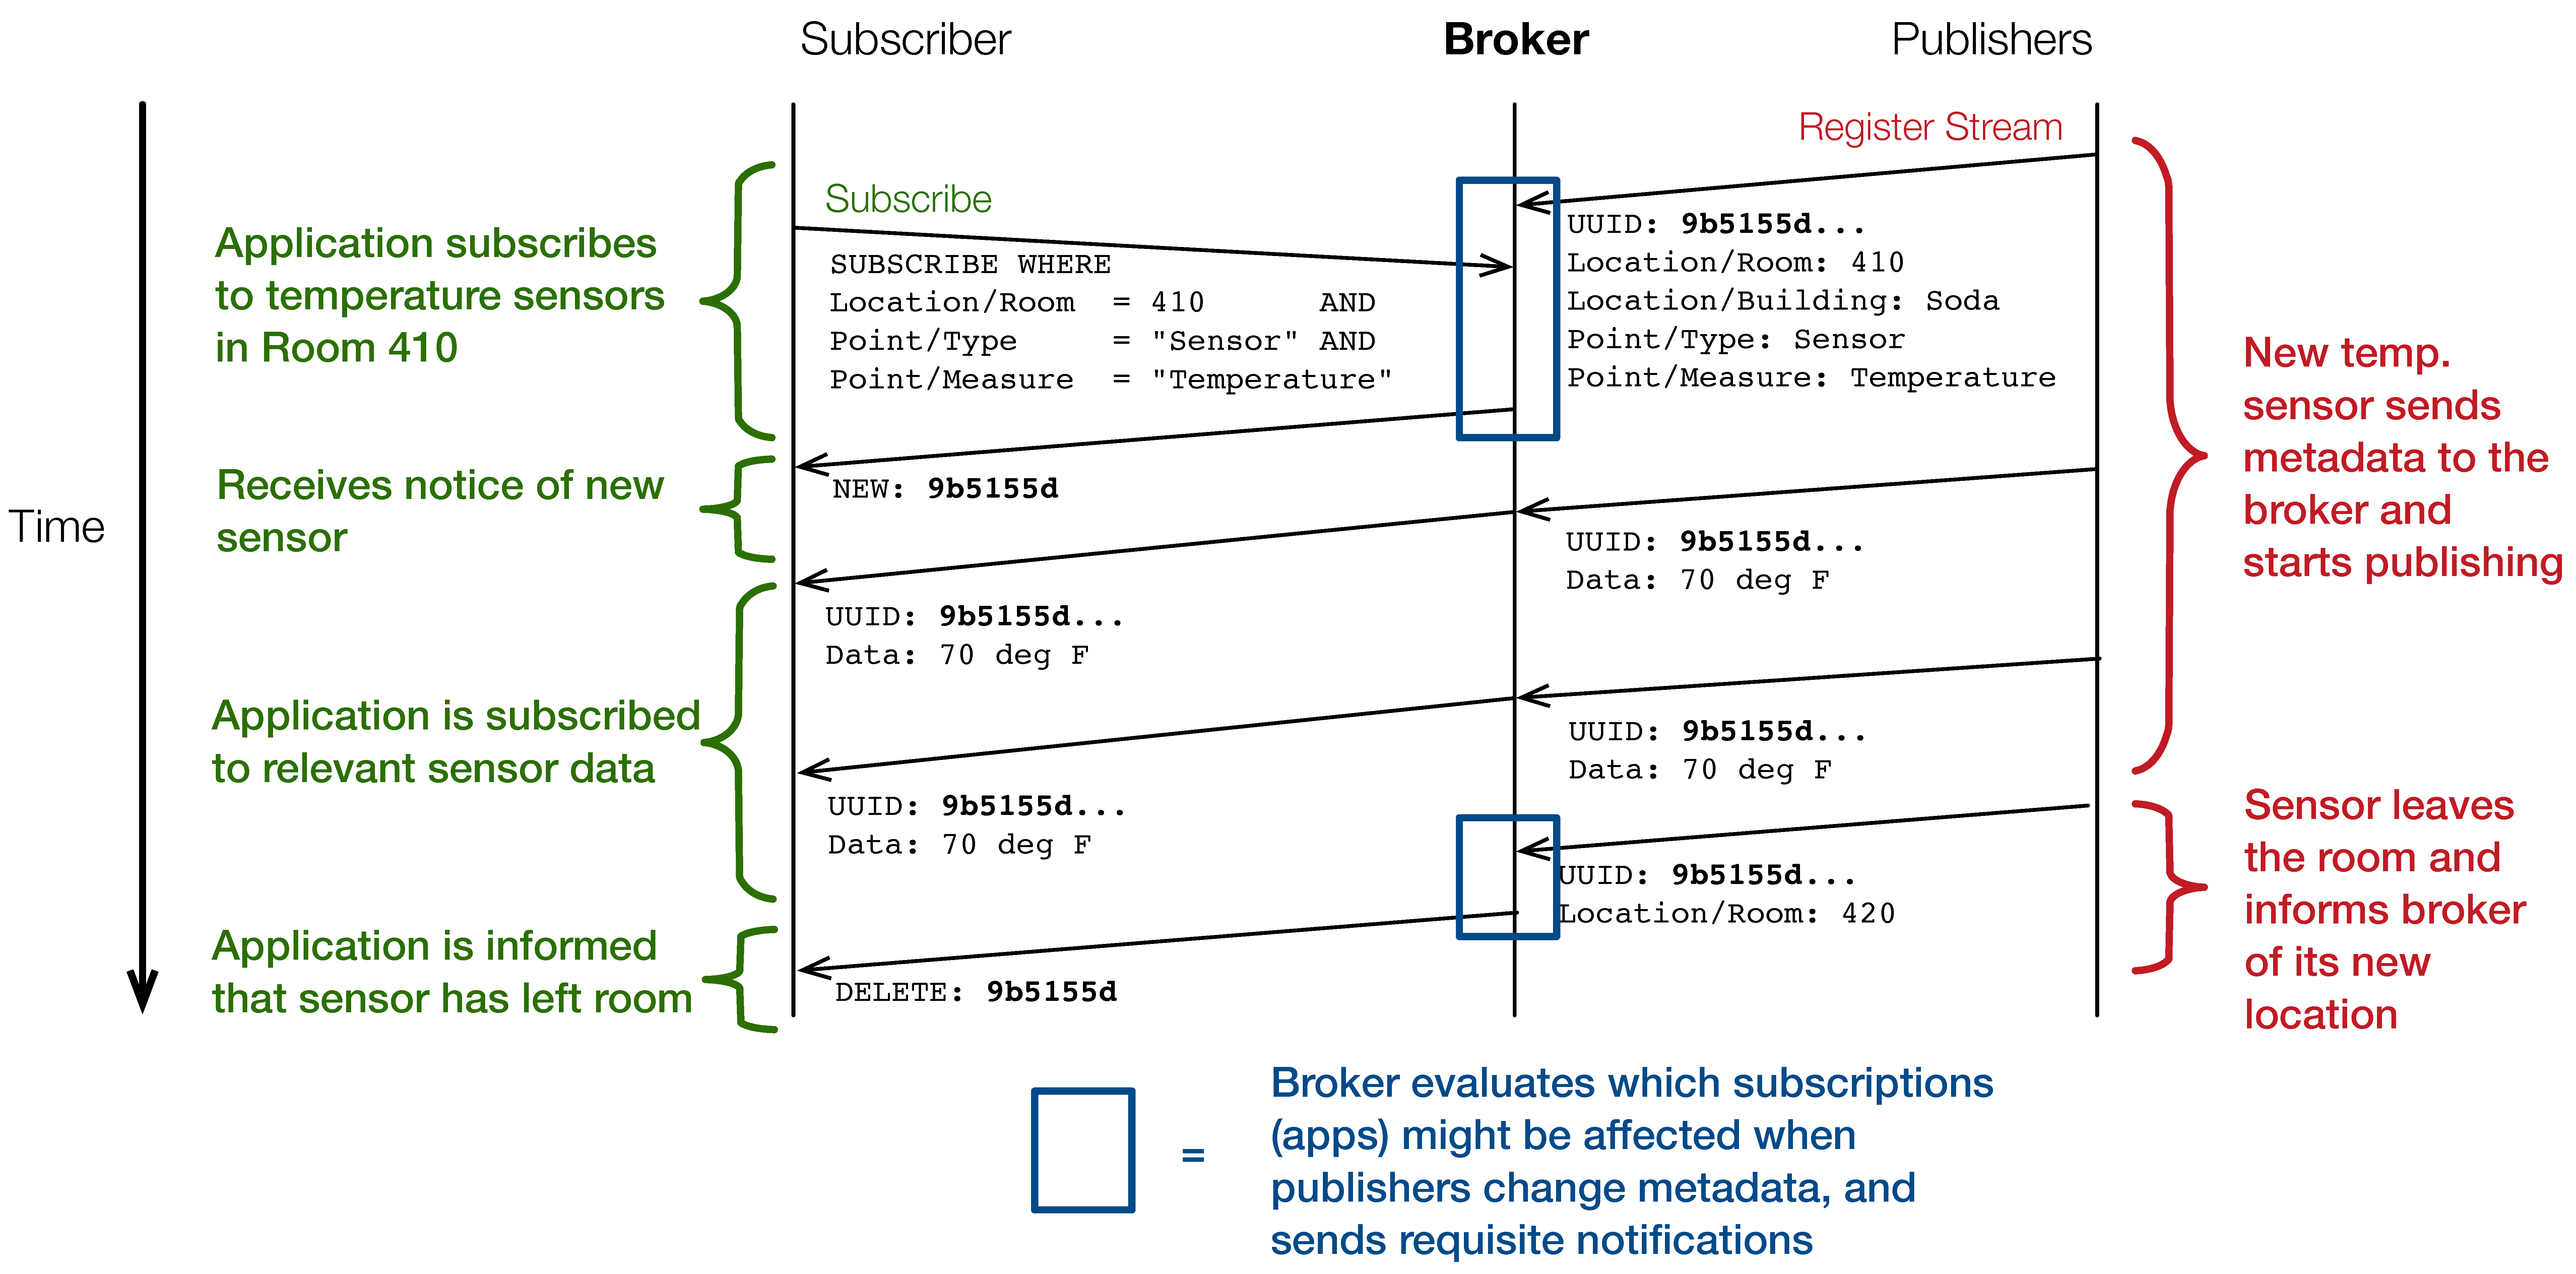
\includegraphics[width=.8\linewidth]{figs/messages.pdf}
\caption{The network traffic for a continuous query for discovering all temperature sensors in room 410 (ommitted
for brevity are additional constrains for building, units, etc). As new streams are registered, or their metadata
changes to no longer fit the discovery constraints, the client is updated in real-time.}
\label{fig:messages}
\end{figure*}
